\section{Grundlagen und Ansätze}

TODO

\subsection{Softwaretests}

TODO

\subsection{Virtualisierung von Testumgebungen}

Laut Duden leitet sich das Adjektiv "`virtuell"' vom lateinischen "`virtus"' für "`Tüchtigkeit, Mannhaftigkeit, Tugend"' ab. Es bedeutet so viel wie "`nicht echt, nicht in Wirklichkeit vorhanden, scheinbar"' \citep[Vgl.][]{duden:001}.

Innerhalb der Informatik spricht man immer dann von Virtualität oder Virtualisierung, wenn einem Benutzer oder einem Softwareprozess eine Umgebung vorgespielt wird, die physisch nicht wirklich existiert.

Der für diese Arbeit interessante Bereich der Virtualisierung ist das Bereitstellen virtueller Betriebsumgebungen. Eine Betriebsumgebung meint die Umgebung, die ein Programm für seine Ausführung benötigt. Dazu gehören vor allem bestimmte Hardware-Bauteile (Prozessoren, Arbeitsspeicher, Festplatten, Netzwerk-Adapter), ein Betriebssystem und eventuell zusätzliche Anwendungsprogramme, mit denen das Programm interagiert. Für gewöhnlich läuft eine solche Betriebsumgebung genau auf einem Rechner (zum Beispiel Server oder Desktoprechner). Mit Hilfe der Virtualisierung ist es nun aber möglich, mehrere solcher Betriebsumgebungen auf dem gleichen Rechner laufen zu lassen. Dabei wird der Betriebsumgebung eben nur vorgespielt, auf einem eigenen Rechner zu laufen \citep[Vgl.][Abstract]{DamMohAnd12}.

Es gibt verschiedene Ziele, die man mit der Virtualisierung von Betriebsumgebungen verfolgen kann. Zum einen lässt sich eine effizientere Nutzung der Ressourcen erreichen. Da die tatsächliche Hardware abstrahiert wird, kann diese durch das hinzufügen weiterer Betriebsumgebungen vollständig ausgenutzt werden. Eine Firma könnte also zum Beispiel für jeden Mitarbeiter eine Arbeitsumgebung auf einem zentralen Server starten. Da diese nur Ressourcen verbraucht, wenn der Mitarbeiter tatsächlich arbeitet, kommt man unterm Strich mit weniger Hardwareressourcen aus, als wenn man jedem Mitarbeiter einen echten eigenen Rechner zur Verfügung stellt. Der Betrieb und die Wartung von virtuellen Arbeitsumgebungen lässt sich dabei auch besser planen und einfacher durchführen. Außerdem ist in den letzten Jahren das Mieten solcher zentralen Hardwareressourcen populär geworden. Man spricht hierbei auch gerne von sogenannten Cloud-Anbietern oder Cloud-Lösungen. In diesem Falle würde die Hardware erst gar nicht eingekauft und selbst betrieben oder gewartet werden. Dies würde dann in den Aufgabenbereich des Dienstleisters fallen, der (oft minutengenau abgerechnet) nur die tatsächliche Nutzung der Ressourcen in Rechnung stellt \citep[Vgl.][S. 7]{ZhaChe14}.

Ein weiteres Ziel der Virtualisierung von Betriebsumgebungen ist die Trennung beziehungsweise Isolierung verschiedener Anwendungen \citep[Vgl.][Abstract]{Schee14}. Statt zum Beispiel auf einem Server einen Datenbankserver zu installieren, in dem mehrere Mitarbeiter oder auch Kunden ihre Datenbanken pflegen, kann man mit Hilfe von Virtualisierungsansätzen einfach für jeden Anwender einen eigenen Datenbankserver laufen lassen. Zwar bieten Datenbankserver natürlich auch innerhalb einer Instanz die Möglichkeit, den Zugriff auf einzelne Datenbanken zu begrenzen. Die Konfiguration solcher Zugriffsberechtigungen kann aber komplex sein und ist somit fehleranfällig. Gerade aus Sicherheitsgründen kann es somit lohnenswert sein, Anwendungen bereits auf Betriebsumgebungsebene voneinander zu trennen. Zudem gibt es Anwendungen, die selbst keine differenzierbaren Zugriffskonzepte kennen und somit so oder so für jeden Anwender separat gestartet werden müssen. Die eingangs beschriebenen Probleme bei der Testausführung für die Anwendung der Webseite Chefkoch.de lassen sich, wie wir später noch einmal im Detail sehen werden, auf solche mangelnde Isolation zwischen den Anwendungsteilen zurückführen.

Die Virtualisierung von Betriebssumgebungen ist aber auch mit Nachteilen verbunden. So geht durch die Virtualisierung Rechenleistung verloren. Ausgeführte Anwendungen sind also mitunter langsamer, als wenn man sie auf echter Hardware betreibt. Die virtualisierten Betriebsumgebungen sind zudem zwar grundsätzlich von einander isoliert. Da sie aber auf der selben Hardware laufen, ist es je nach Virtualisierungstechnik sehr schwer sicherzustellen, dass sie sich garnicht beeinflussen. Auch im Bereich des Datenschutzes und der Lizensierung von Softwareprodukten kommen durch Virutalisierungslösungen neue Probleme auf. So richten sich viele Lizensmodelle nach Anzahl der physischen Prozessoren und der Größe des physischen Arbeitsspeichers. Beides kann aber bei der Virtualisierung nicht zwangsläufig genau einer Betriebsumgebung und deren Anwendungen zugeordnet werden.

Es gibt nun verschiedene Ansätze, Betriebsumgebungen zu virtualisieren. Grundsätzlich unterscheidet man hinsichtlich ihrer Funktionalität und Implementierung zwischen der Systemvirtualisierung mittels Hypervisor und der Betriebssystemvirtualisierung mittels OS-Containern. Auf diese Varianten soll nun im Näheren eingegangen werden.

\begin{figure}[!ht]
  \begin{center}
    \includegraphics[width=8cm]{bilder/Einordnung_Virtualisierungstechnologien_für_virtuelle_Betriebsumgebungen.png}
    \caption{Einordnung Virtualisierungstechnologien für virtuelle Betriebsumgebungen \citep{Hirschbach06}}
  \end{center}
\end{figure}

\subsubsection{Systemvirtualisierung mittels Hypervisor}

Als Hypervisor oder auch \ac{VMM} wird eine Software bezeichnet, die die physisch vorhandene Hardware abstrahiert und mehreren Gastbetriebssystemen zur Verfügung stellt. Dabei spielt es den Gastsystemen jeweils vor, dass sie auf einem eigenen vollständigen Rechner mit Prozessor, Arbeitsspeicher, Festplatte und sonstigen Geräten laufen. Ein solcher virtueller Rechner wird auch \ac{VM} genannt \citep[Vgl.][S. 413]{PopGol74}.

Um die Herausforderung dieses Virtualisierungsansatzes genauer zu verstehen, ist es notwendig, sich die Prozessorarchitektur heutiger Desktop- und Serverrechner anzuschauen. Im Falle der Infrastruktur der Webseite Chefkoch.de ist dies - wie auch in einer Vielzahl anderer Umgebungen - die Familie der X86-Prozessoren (32bit) beziehungsweise deren 64bit Erweiterung AMD64. Solche Prozessorarchitekturen beschreiben vor allem eine bestimmte Menge an Befehlssätzen, die der vom Prozessor ausgeführte Programmcode aufrufen kann, um bestimmte Operationen auszuführen. Solche Befehlssätze beinhalten zum Beispiel Befehle zum Kopieren von Daten innerhalb des Systems (Transferbefehle) oder auch arithmetische Befehle zur Verrechnung von Werten. Die X86-Architektur unterstützt nun das Konzept sogenannter Ringe. Ein Ring bezeichnet dabei eine Sicherheitsstufe eines Prozesses, der vom Prozessor verarbeitet wird. Je nach Sicherheitsstufe darf der Prozess dabei auf mehr oder weniger Befehlssätze innerhalb des Prozessors zugreifen. Der Ring 0 bezeichnet dabei die Sicherheitsstufe, innerhalb derer ein Prozess auf alle Befehlssätze des Prozessors zugreifen darf. Man nennt diesen Ring auch "`Kernel-Mode"', da in diesem Modus typischerweise nur das Betriebssystem beziehungsweise dessen Kern, der sogenannter Kernel, ausgeführt wird. Prozesse normaler Anwendungsprogramme werden hingegen in Ring 3 ausgeführt, der nur wenige Befehlssätze ausführen darf. Man nennt diesen Ring auch "`User-Mode"'. Ein Prozess im Ring 3 darf zum Beispiel keine Transferbefehle ausführen. Benötigt er entsprechende Operationen, greift er auf Funktionen des Kernels des Betriebssystems zu, die dabei bestimmte Berechtigungen sicherstellen können. Ein Prozess in Ring 3 kann somit zum Beispiel nicht auf den Arbeitsspeicher anderer Prozesse zugreifen oder sich selbst in einen anderen Ausführungsmodus bringen. Würde ein Prozess in Ring 3 auf einen nicht erlaubten Befehl zugreifen, so löst der Prozessor eine Exception aus, die vom Kernel beziehungsweise vom Programm-Code in Ring 0 aufgelöst werden muss, indem er zum Beispiel einen alternativer Befehl zur Ausführung bringt oder den betroffenen Prozess zur Not beendet.

\begin{figure}[!ht]
  \begin{center}
    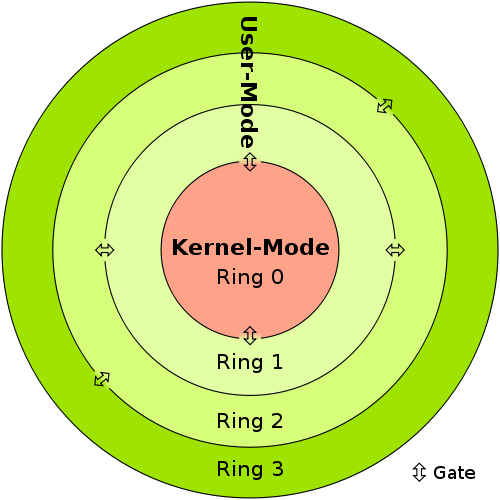
\includegraphics[width=6cm]{bilder/500px-CPU_ring_scheme.png}
    \caption{CPU Ring scheme \citep{wiki:006}}
  \end{center}
\end{figure}

Um nun mit Hilfe der Virtualisierung mehrere Betriebssysteme nebeneinander auszuführen, die sich gegenseitig nicht beeinflussen können, ist es notwendig, deren Kernel nicht im Ring 0, sondern in einem höheren Ring mit weniger Berechtigung auszuführen. Da der Programm-Code des Gast-Kernels dabei natürlich dennoch Befehle rufen würde, die nur in Ring 0 ausführbar sind, kommt es zu den eben beschriebenen Exceptions. Die Lösung dieser Ausnahmesituationen ist dabei nun Aufgabe des Hypervisors. Dazu beinhaltet ein Hypervisor immer mindestens einen Prozess, der selbst in Ring 0 läuft und in der Lage ist, die Auflösung der Ausnahmesituationen zu erledigen. Ein Hypervisor kann dabei nun verschiedene Strategien anwenden. Die einfachste Strategie ist eben, auf entsprechende Exceptions zu warten und diese zum Beispiel durch Aufrufe auf das eventuell vorhandene Host-Betriebssystem oder den Ring-0-Prozess des Hypervisors zu ersetzen. Auch wenn diese Strategie funktioniert, so ist die Behandlung tausender solcher Ausnahmesituationen sehr teuer und beinträchtigt die Leistung des Gastsystems empfindlich. Moderne Hypervisoren verfolgen deshalb eine zwar sehr viel kompliziertere aber eben auch effizientere Strategie. Sie scannen den Programm-Code des Gastsystems nach problematischen Befehlen und ersetzen diese bereits vor der Ausführung im Speicher mit Befehlen, die in der Berechtigungsstufe des Gastsystems erlaubt sind. Heutige Prozessoren kennen mitunter sogar das Konzept der Virtualisierung mittels Hypervisor und bieten spezielle Befehlssätze an, die sich besonders für diese Ersetzung eignen und sich aus eingeschränkten Berechtigungsstufen rufen lassen. Moderne Hypervisoren und Betriebssysteme kommen damit auf Ausführungszeiten, die nahezu denen auf direkter physischer Hardware entsprechen.

Die obige Beschreibung der Herausforderungen bei der Virtualisierung auf Basis der Prozessorarchitektur x86 stützen sich vor allem auf die Seiten 203-206 des Oracle VM VirtualBox User Manuals \citep{Oracle14}.

Robert P. Goldberg, der die Grundlagen des \ac{VMM} in den 70er Jahren wissenschaftlich erarbeitet hat, unterscheidet in seiner Doktorarbeit "`Architectural Principles for Virtual Computer Systems"' nun zwei Klassen des \ac{VMM} \citep[vgl.][S. 22 ff.]{Goldberg73}: Dem Typ I \ac{VMM} oder auch "`Bare Metal Hypervisor"' und dem Typ II \ac{VMM} oder auch "`Hosted Hypervisor"'. In den folgenden beiden Unterkapiteln sollen diese beiden Klassen und entsprechende Implementierungen näher beleuchtet werden.

Darauf folgt abschließend ein Unterkapitel zu den sogenannten Unikernels, einer relativ neuen Entwicklung innerhalb der Systemvirtualisierung mittels Hypervisor, die eine bestimmte Art von \ac{VM} beschreibt.

\subsubsubsection{Bare Metal Hypervisors}

Ein Bare Metal Hypervisor ist ein \ac{VMM}, der als eigenständiges Programm direkt auf echter physischer Hardware läuft und somit kein Betriebssystem auf dem Hostsystem benötigt.

\begin{figure}[!ht]
  \begin{center}
    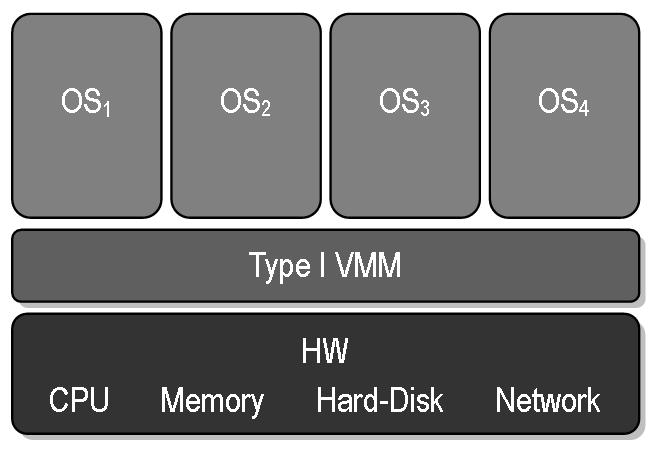
\includegraphics[width=6cm]{bilder/VMM-Type1.jpg}
    \caption{Virtual Machine Monitor Type I \citep{wiki:002}}
  \end{center}
\end{figure}

Durch diesen direkten Zugriff und das nicht notwendige Hostbetriebssystem gilt ein Bare Metal Hypervisor als ressourceneffizienter als ein Hosted Hypervisor. Größter Nachteil dieser Variante ist aber, dass sie mit mehr Installationsaufwand verbunden ist, da der Hypervisor selbst die passenden Gerätetreiber für die zugrundeliegende Hardware benötigt und man nicht auf Standardwerkzeuge wie zum Beispiel den Installationsmanagers eines Hostbetriebssystems zugreifen kann. Typische Vertreter dieser Hypervisor-Klasse sind zum Beispiel VMWare vSphere, KVM und Citrix XenServer.

\begin{figure}[!ht]
  \begin{center}
    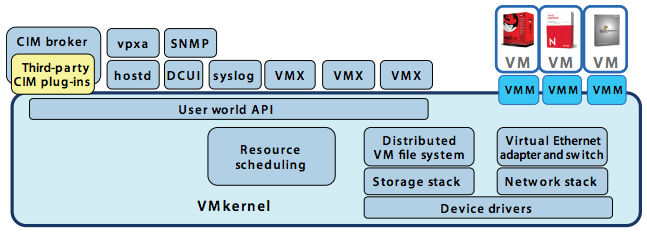
\includegraphics[width=10cm]{bilder/vmware.png}
    \caption{VMWare vSphere Architektur \citep{vmware:002}}
  \end{center}
\end{figure}

Bei VMWare vSphere handelt es sich um ein kommerzielles Produkt der Firma VMWare, dem Marktführer im Bereich der Virtualisierungslösungen mit einem Marktanteil von ungefähr 50\% \citep[vgl.][]{vmware:001}. vSphere basiert auf einem von WMWare eigens entwickelten Betriebssystem, dem sogenannten VMkernel. Auf diesem Betriebssystem laufen das Programm DCUI (Direct Console User Interface), eine Konsole zur direkten Konfiguration des Servers, und diverse weitere Schnittstellen, mit denen man die Verwaltung des Servers und der auf ihm laufenden virtuellen Maschinen auch über das Netzwerk erledigen kann. Für jede virtuelle Maschine wird ein eigener Hypervisor- und ein weiterer Hilfsprozess gestartet (VMM und VMX). vSphere bietet die Möglichkeit, virtuelle Maschinen im laufenden Betrieb von einem vSphere Server auf einen anderen zu übertragen. Diese Funktion, vMotion genannt, erleichtert das Resourcenmanagement enorm, da sich eine laufende Anwendung auf andere Hardware übertragen lässt, um die vorherige Hardware zum Beispiel zu reparieren oder auch einfach nur zur Einsparung auszuschalten.

\begin{figure}[!ht]
  \begin{center}
    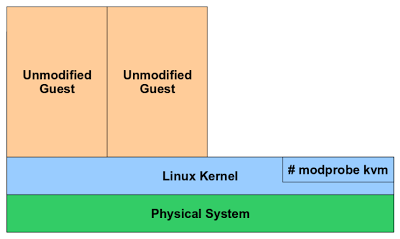
\includegraphics[width=8cm]{bilder/kvm.png}
    \caption{KVM Architektur \citep{kvm:002}}
  \end{center}
\end{figure}

Beim Open-Source-Produkt KVM (Kernel-based Virtual Machine) handelt es sich um eine Lösung, bei der ein normaler Linux-Kernel über ein spezielles Kernel-Modul für die grundsätzliche Virtualisierung (kvm.io) und ein weiteres prozessorspezifisches Kernel-Modul (kvm-intel.io oder kvm-amd.io) in die Lage versetzt wird, als Hypervisor zu arbeiten und Gastsysteme zu verwalten. KVM lässt sich damit grundsätzlich auf allen gängigen Linux Distributionen installieren. Oft wird deshalb vermutet, dass es sich nicht um einen reinen Bare Metal Hypervisor handelt, da er eben zusammen mit einem Betriebssystem installiert wird. Da es sich bei dem Kernel-Modul aber nicht um ein Anwendungsprogramm handelt, sondern um eine Erweiterung des eigentlichen Kernels, setzt diese Virtualisierungslösung direkt auf der darunterliegenden Hardware und nicht auf einem dazwischenliegenden Kernel auf \citep[Vgl.][S. 225 - 227]{KivKam07}.

So gibt es zum Beispiel die Linux Distribution Proxmox VE, die man direkt auf eine leere Hardware installieren kann und die die entsprechenden Kernel-Module und weitere Hilfsprogramme (zum Beispiel zur Verwaltung der virtuellen Maschinen) bereits beinhaltet \citep[Vgl.][]{Proxmox14}.

\begin{figure}[!ht]
  \begin{center}
    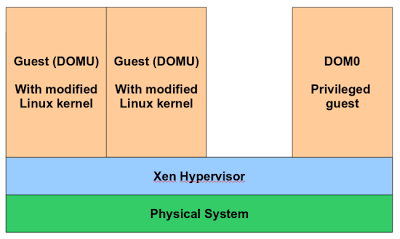
\includegraphics[width=8cm]{bilder/xen.png}
    \caption{Xen Architektur \citep{kvm:002}}
  \end{center}
\end{figure}

Auch bei XenServer von der Firma Citrix handelt es sich um ein Open-Source-Produkt. Auch dieser \ac{VMM} setzt direkt auf der eigentlichen physischen Hardware auf. XenServer basiert ebenfalls auf einem Linux-Kernel. Es handelt sich aber nicht lediglich um Kernel-Module, die sich in eine beliebige Linux-Distribution laden lassen, sondern um einen modifizerten Linux-Kernel. XenServer lässt sich also nur auf komplett leere Hardware installieren und bietet auch nicht die vollständigen Funktionalitäten einer normalen Linux-Distribution. Das besondere an XenServer ist, dass die Prozesse zur Steuerung der virtuellen Maschinen selbst in einer virtuellen Maschine laufen. Diese auch "`Privileged Guest"' genannte Maschine muss laufen, bevor weitere Gastsysteme geladen werden können. Der "`Privileged Guest"' oder auch DOM0 genannte Gast hat dabei (wie der Name sagt) besondere Rechte, die ihm die Steuerung der darunterliegenden Virtualisierungsschicht im Hypervisor ermöglichen \citep[Vgl.][S. 2]{Schee14}.

Als weitere Gastsysteme lassen sich wie auch bei KVM beliebige unmodifzierte Gastsysteme wie Linux-Distributionen oder Windows-Systeme installieren. Besonders ist aber, dass sich auch Linux-Distributionen mit ebenfalls modifiziertem Kernel laden lassen, die direkter mit dem Hypervisor zusammen arbeiten und so eine höhere Performance bieten.

\subsubsubsection{Hosted Hypervisors}

Ein Hosted Hypervisor ist ein \ac{VMM}, der als Anwendungsprogramm innerhalb eines Hostbetriebssystems läuft. Es ist somit möglich, auch andere Programme neben dem Hypervisor und seinen Gastbetriebssystemen zu verwenden.

\begin{figure}[!ht]
  \begin{center}
    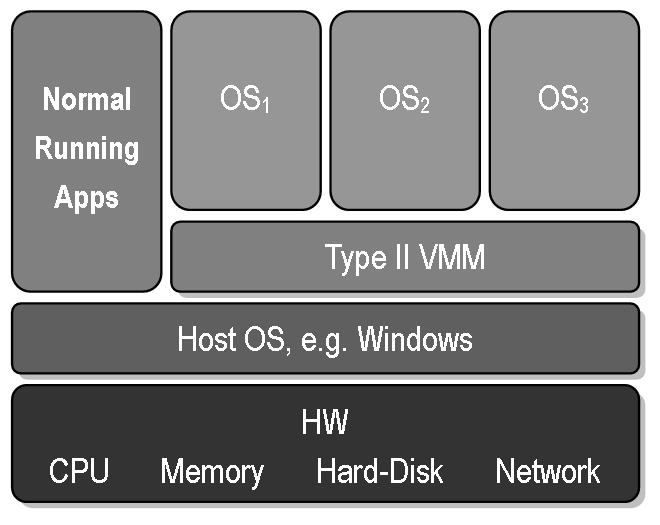
\includegraphics[width=6cm]{bilder/VMM-Type2.jpg}
    \caption{Virtual Machine Monitor Type II \citep{wiki:003}}
  \end{center}
\end{figure}

Größter Vorteil dieser Variante ist es also, dass das Hostsystem auch für gewöhnliche Benutzerarbeiten zur Verfügung steht und nicht ausschließlich zur Virtualisierung verwendet werden muss. Diese Virtualisierungslösung lässt sich sehr einfach nachträglich auf eine Vielzahl von Betriebssystemen installieren und auch wieder deinstallieren. Ein typischer Vertreter dieser Hypervisor-Klasse ist zum Beispiel VirtualBox von Oracle \citep[Vgl.][S. 24]{DamMohAnd12}.

VirtualBox bietet nach der Installation eine grafische Benutzeroberfläche, mit der man seine virtuellen Maschinen einfach verwalten kann. Zum Beispiel ist es möglich, eine neue, leere virtuelle Maschine zu definieren, ihre Hardware-Einstellungen wie zum Beispiel Menge an Prozessoren und Arbeitsspeicher zu konfigurieren und sie zu starten. Anschließend lässt sich dann zum Beispiel mit einem Installationsmedium ein Betriebssystem auf der Gast-Maschine installieren. Es lassen sich aber auch bestehende Maschinen exportieren und importieren, auf denen zum Beispiel bereits ein Betriebssystem und weitere Anwendungsprogramme installiert sind. Schließlich lassen sich virtuelle Maschinen auch einfach pausieren, stoppen und natürlich löschen \citep[Vgl.][S. 11 ff.]{Oracle14}.

\begin{figure}[!ht]
  \begin{center}
    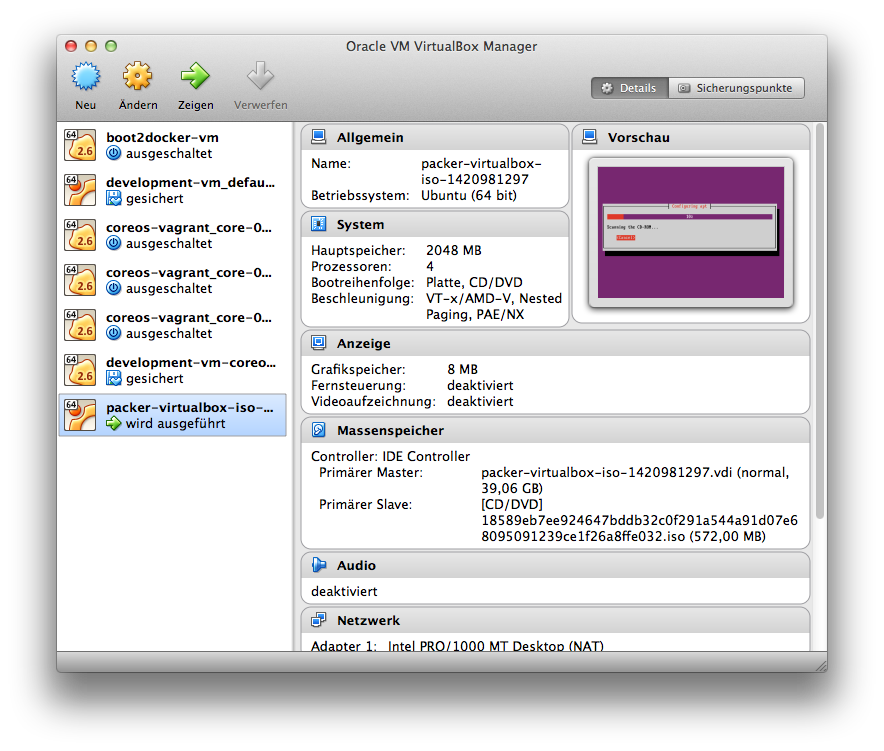
\includegraphics[width=8cm]{bilder/virtualbox-gui.png}
    \caption{Grafische Benutzeroberfläche von VirtualBox}
  \end{center}
\end{figure}

Neben der grafischen Benutzeroberfläche bietet VirtualBox aber auch alle Funktionen in Form von Kommandozeilen-Programmen an. Damit lässt sich VirtualBox auch leicht automatisiert verwenden, zum Beispiel von einem Continuous-Integration-Server aus, der Testumgebungen starten möchte \citep[Vgl.][S. 113]{Oracle14}.

\subsubsubsection{Unikernels}

Eine relativ neue Entwicklung innerhalb der Systemvirtualisierung mittels Hypervisor sind die sogenannten Unikernels. Vertreter dieser Idee kommen zum Beispiel aus dem Bereich der \ac{SOA} oder der Microservice Architecture. In diesen Architekturen wird versucht, die Teile eines IT-Systems als einzelne Dienste zu betrachten, die (meist über Netzwerk) miteinander kommunizieren. Es ist dabei von Vorteil, wenn diese Dienste jeweils eine bestimmte Aufgabe erledigen und über eine einfache Schnittstelle angesprochen werden können. Solche Dienste können nun jeweils über eine eigene \ac{VM} innerhalb der Virtualisierung abgebildet werden. Hierbei wird nun kritisiert, dass die Installation eines kompletten Gastbetriebssystems und die in ihm laufenden Anwendungsprogramme meist wesentlich mehr Resourcen und Programmcode verwenden und mehr Zugriffspunkte bieten, als für den eigentlichen Dienst benötigt wird. Als konzeptionelles Beispiel stellen wir uns hier einmal einen Dienst vor, der als einzige Aufgabe hat, mit Hilfe einer fortlaufenden Zahl neue Kundennummern zu generieren. Es ist nun durchaus nachvollziehbar, dass ein komplettes Gastbetriebssystem inkl. aller in ihm installierten Zubehörprogramme, Dokumentationen und Treiber sehr viel mehr Resourcen verbraucht, als für die eigentliche Operation sinnvoll erscheint. Die höhere Menge an Quellcode und typische Betriebssystemschnittstellen stellen zudem auch ein erhötes Sicherheitsrisiko dar, da sie potentiell mehr Angriffsvektoren bieten \citep[Vgl.][Abstract und Introduction]{MadMorAnd13}.

\begin{figure}[!ht]
  \begin{center}
    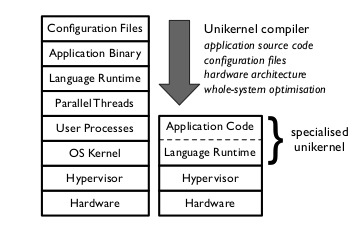
\includegraphics[width=8cm]{bilder/comparison-vm-unikernel.png}
    \caption{Vergleich klassische VM und Unikernel \citep[Abb. 1]{MadMorAnd13}}
  \end{center}
\end{figure}

Als Antwort entstehen deshalb in jüngster Vergangenheit neue Lösungen, bei denen man seinen eigentlichen Programmcode mit Hilfe einer Library entwickelt, die einfache Schnittstellen zur Verfügung stellt, um zum Beispiel Netzwerkkommunikation oder ähnliches zu betreiben. Der Programmcode wird dann mit Hilfe dieser Library in eine sehr viel kleinere \ac{VM} kompiliert, die wieder mit Hilfe eines Hypervisors ausgeführt werden kann. Ein Beispiel für eine solche Library ist MirageOS \citep[Vgl.][]{MadMorAnd13}.

Ein Nachteil dieser Lösung ist, dass man lediglich Funktionalität wiederverwenden kann, die genau durch die benutzte Library zur Verfügung steht. So kann man auch lediglich in der Programmiersprache arbeiten, die der Compiler der Library versteht. Im Falle von MirageOS ist dies die Sprache Ocaml. Es ist somit zum Beispiel nicht möglich, einen PHP-Interpreter zu starten und PHP-Scripte auszuführen, wie das mit allen gängigen Betriebssystemen wie Linux, MacOS oder Windows der Fall ist. Unikernels lassen sich somit zumindest bisher nur für sehr spezielle Dienste und Problemestellungen einsetzen.

\subsubsection{Betriebssystemvirtualisierung mittels OS-Containern}

Ein ganz anderer Ansatz als die Systemvirtualisierung mittels Hypervisor ist die sogenannte Betriebssystemvirtualisierung mittels OS-Container. Dabei wird nicht versucht, ein komplettes Gastsystem mit eigener, virtualisierter Hardware und eigenem Kernel auszuführen. Vielmehr basiert dieser Ansatz darauf, dass sich alle virtuellen Betriebssysteme die Hardware und einen gemeinsamen Kernel teilen. Offensichtlich lassen sich damit nicht verschiedenste Betriebssysteme auf einer Maschine virtualisieren, sondern immer nur Betriebssysteme, die auf dem gleichen Kernel basieren wie das Hostsystem. Dafür entfällt die Notwendigkeit, Hardware zu emulieren oder zu virtualisieren. In Bezug auf das Ring-Schemas des Prozessors gilt: Der gemeinsame Kernel arbeitet im Ring 0 und somit direkt auf der physischen Hardware. Das virtualisierte System beinhaltet lediglich Bibliotheken und Anwendungsprogramme und arbeitet somit in Ring 3. Die Notwendigkeit, nicht erlaubte Aufrufe zu finden und zu behandeln entfällt damit. Eine solche isolierte Umgebung, OS-Container genannt, gilt damit als grundsätzlich effizienter als komplette virtuelle Maschinen \citep[Vgl.][Introduction]{Turnball14}.

\begin{figure}[!ht]
  \begin{center}
    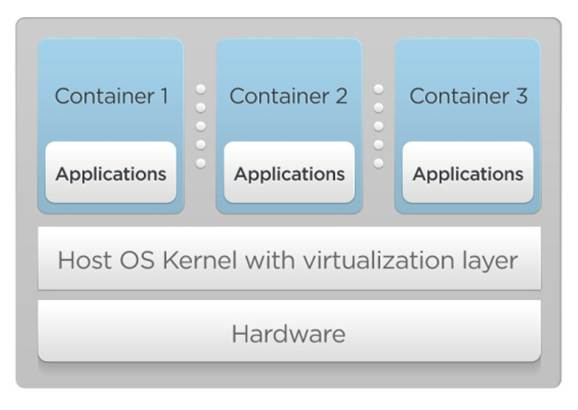
\includegraphics[width=8cm]{bilder/lxc-architecture.jpg}
    \caption{OS-Container \citep{Francis2014}}
  \end{center}
\end{figure}

Damit die einzelnen Container dennoch isoliert laufen und weder das Hostsystem noch andere Container manipulieren können, muss der Kernel spezielle Schnittstellen anbieten. Entsprechende Technologien sind im Laufe der Zeit bei einer Reihe von Betriebssystemen entwickelt worden, zum Beispiel auch für Linux und Windows. Für andere Betriebssysteme wiederum existiert keine entsprechende Schnittstelle, zum Beispiel Mac OS.

Ein prominenter Vertreter dieser Virtualisierungs-Art ist zur Zeit das Produkt Docker. Docker ist eine Open-Source-Plattform, mit deren Hilfe eine einfache Definition und Verwaltung solcher Container für den Linux-Kernel möglich ist. Kürzlich wurde aber auch eine Kooperation zwischen Microsoft und der Docker Inc., dem Unternehmen hinter Docker, bekannt gegeben. Ziel der Kooperation ist es unter anderem, dass sich entsprechende Container auch für Windows-Betriebssysteme erstellen lassen \citep[Vgl.][]{heise:001}.

Docker setzt auf eine Reihe von Schnittstellen auf, die inzwischen Teil des offizielen Linux-Kernels sind. Unter anderem gehören dazu die Cgroups und die Namespaces:

Cgroups (Control Groups) bieten die Möglichkeit, die Ressourcen-Nutzung bei der Ausführung von Prozessen durch den Kernel einzugrenzen. So lassen sich für Prozesse bestimmte Grenzen der Arbeitsspeicher- und Prozessor-Nutzung definieren. Außerdem lassen sich solche Prozesse auch komplett stoppen beziehungsweise pausieren und wieder starten \citep[Vgl.][S. 3]{Schee14}.

Kernel Namespaces erlauben es, die Sichtbarkeit von Prozessen untereinander einzugrenzen. So können über Namespaces zum Beispiel die Prozess-Identifikatoren (PIDs) für jeden Container neu vergeben werden. Jeder Container kann somit einen Prozess mit der ID 1 besitzen. Aber auch andere Aspekte des Betriebssystems, wie zum Beispiel Hostname, Benutzer-IDs, Dateisystem und Netzwerk-Zugriffe lassen sich mit den Kernel Namespaces voneinander trennen \citep[Vgl.][S. 3]{Schee14}.

Docker bietet zusätzlich ein weiteres nützliches Feature, sogenannte Union-Filesystems:

\begin{figure}[!ht]
  \begin{center}
    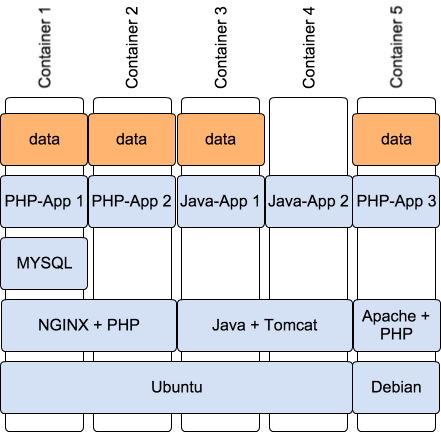
\includegraphics[width=8cm]{bilder/UnionFilesystem.png}
    \caption{Union Filesystem}
    \label{Union Filesystem}
  \end{center}
\end{figure}

Union-Filesystems sind Dateisysteme, die es erlauben, Dateisysteme transparent übereinander zu legen, um so weniger Speicherplatz zu verbrauchen. Das zugrundeliegende Verfahren nennt sich Copy-On-Write. Verwenden zwei Container zum Beispiel die gleiche Linux-Distrubution, so werden die entsprechenden Libraries und Anwendungsprogramme nur einmal auf der Festplatte vorgehalten. Das entsprechende Dateisystem wird dabei read-only unter ein für den Container beschreibbares Dateisystem gelegt. Die beiden Container unterscheiden sich also auf der Festplatte nur durch die tatsächlich individuell von ihnen geschriebenen Daten. Die meisten Union-Filesysteme erlauben dabei ein mehrfaches Übereinanderlegen, so dass eine ganze Hierarchie an ineinander verschachtelten Dateisystemen entstehen kann, um die Unterschiede zwischen den einzelnen Containern maximal effizient auf der Festplatte abzulegen \citep[Vgl.][S. 3]{Schee14}.

In der Abbildung \ref{Union Filesystem} wird zum Beispiel die gesamte Ubuntu-Distribution nur einmal auf der Festplatte abgelegt, obwohl sie von vier laufenden Containern verwendet wird. Sämtliche Dateisysteme sind read-only, bis auf die in rot angedeuteten Kästen, in denen die Container Laufzeitdaten speichern. Container 4 schreibt aber zum Beispiel keine Daten und ist somit komplett nur lesend.

\subsubsection{Vergleich der Virtualisierungsansätze}

TODO
